\chapter{Efficiency calculations}
\label{sec:Efficiency}

The reconstruction steps described in the Section~\ref{sec:Reconstruction} are not absolutely effective. The algorithms occasionally misinterpret particles and thus introduce the errors in the results. This margin of error is called the efficiency, and it is present for reconstructing both collision and MC samples. But to be able to compare collision data to theoretical predictions, the efficiency in both cases should be the same, which is not the case. To remedy this, the so-called "efficiency correction factors" were introduces for every step of the reconstruction chain: for trigger efficiency ($\varepsilon_\mathrm{TG}$), reconstruction efficiency ($\varepsilon_\mathrm{Reco}$), identification efficiency ($\varepsilon_\mathrm{ID}$), and isolation efficiency ($\varepsilon_\mathrm{ISO}$). The correction factor for every efficiency is defined as a ratio $\varepsilon^\mathrm{data}/\varepsilon^\mathrm{MC}$.

All efficiencies are measured using the tag-and-probe method, which require two electrons, one of which should pass the tight identification and would be called "tag", and the other should pass the weak identification and would be called "probe". If the "probe" also passes the tight identification, it is called "passing probe", and it is called "failing probe". The efficiency is then calculated as a ratio of the passing probes to the whole amount of tags, and is usually calculated in 2D binning of $|\eta|$ and \pt.

In the following sections all the efficiencies would be discussed separately.

\section{Trigger efficiency}

The efficiency of the electron triggers was determined with the help of the \Zee\ data which gives a clear selection of electrons with wide range in both \pt\ and $\eta$. For the central-forward analysis one uses a single-electron trigger, but since we need two electrons for the tag-and-probe method, the trigger efficiency was calculated using the central-central \Zee\ data. To get that data, the usual \Zee\ CC cut chain was applied, but with identification (ID) and isolation (ISO) cuts being changed to that, required from the central electrons from the \Zee\ CF and \Wenu\ analyses. After that every electron was consecutively used as a "tag" and as a "probe", with the "tag" always being required to be matched to the single-electron trigger, and the efficiency of a successful match of the "probe" to the same trigger being evaluated.

The scale factors were calculated in three different mass windows of $70 \le m_{ee} \le 110$~GeV, $80 \le m_{ee} \le 100$~GeV, and $85 \le m_{ee} \le 95$~GeV, to vary the background level. The results from the middle mass window were used to define the central value of the scale factors, while the other two were used to derive a source of uncertainty. To evaluate the uncertainty further, a background subtraction via OS-SS pairs (opposite sign minus same sign) was performed. The central value was taken from the OS pairs and the full difference to the OS-SS sample was taken as another source of uncertainty.

The whole MC sample was divided into four periods, corresponding to data periods B-H, I-J, K and L-M. Each of these MC periods is distinguishable by its unique LAr calorimeter and trigger setups, and should be used separately in order to calculate the scale factors which are valid only for that particular period. After propagation to the final cross section measurement using the combined ToyMC method (see Section~\ref{sec:ZeeD_toymc}), the resulting uncertainty is typically $0.1\%$ only.

The calculated trigger efficiencies as function of $\pt$ and $\eta$ for the default single-electron triggers used in the analysis are presented in Figure~\ref{fig:eff_trig}.

\begin{figure}
\center{
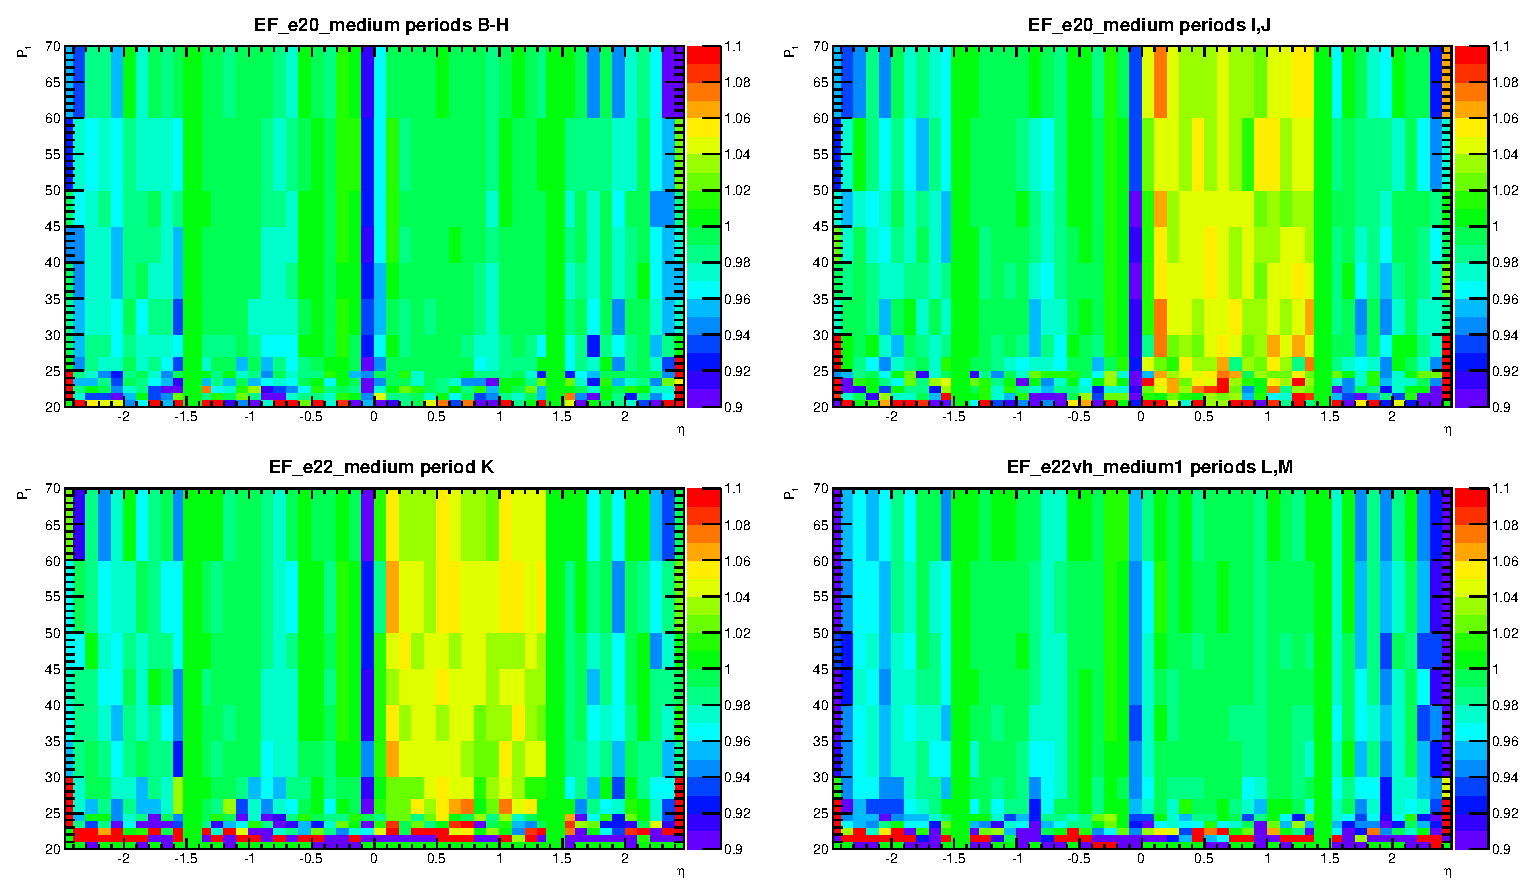
\includegraphics[width=1.0\textwidth]{figures/SingElTrigSFs2D.eps}
\caption{Scale factors for the default single-electron triggers used in the 2011 data. The plots were made using the \Zee\ MC samples with standard CC analysis cuts with the additional requirements on electron ID and ISO from the CF analysis.}
\label{fig:eff_trig}}
\end{figure}

\section{Reconstruction and identification efficiency}

There are three separate efficiencies that contribute to the electron identification: the efficiency of the cluster reconstruction algorithm, the efficiency of the electron reconstruction algorithm, and the efficiency of the electron identification algorithm. Every subsequent algorithm only works if its predecessors succeeded, so all the three efficiencies are tied together, and may be explored together.

\subsection{Central electron identification efficiencies}

For the central electrons, the samples from the \Zee, \Wenu, and $J/\psi \to ee$ were taken in the kinematic intervals of $7 < \et < 50$~GeV and $|\eta| < 2.47$~\cite{lib:elec_reco}. The efficiencies and uncertainties were calculated separately for each channel, and then combined for the calculation of the scale factors to reduce the uncertainties. For all three channels the selection for the tag electron required it to be reconstructed inside the $|\eta| < 2.47$ range with at least six hits in the SCT and at least one hit in the pixel detector. Tight selection criteria are applied to the tag object, which is an electron in case of \Zee\ and $J/\psi \to ee$ events, and is a $\et^{miss}$ in case of \Wenu. To further decrease the amount of background, additional cuts were applied to each channel separately.

For the \Wenu\ channel the selection was tighten for the lower-mass events, i.e. the ones with the transverse energy $40 < \et < 50$~GeV and missing transverse energy $25 < \et^{miss} < 40$~GeV. For the tighter selection, the probe electron was required a $\pt > 15$~GeV, and the event was discarded if more then one electron candidate satisfied the medium ID criteria. To reduce the amount of hadrons misidentified as electrons, two additional isolation criteria were added: the probe electron should be separated from any jet with $\pt > 25$~GeV with a cone of at least $\Delta R > 0.4$, and similarly the $\et^{miss}$ vector should be separated from any jet with the same energy by the angular distance of at least $\Delta \varphi > 0.7$.

For the \Zee\ channel the additional criteria included the $\et > 20$~GeV cut for the tag electron, as well as exclusion of the transition region $1.37 < |\eta| < 1.52$, and similar to isolation requirement for the probe electron from the \Wenu channel: no jets with $\pt > 25$~GeV within the $\Delta R < 0.4$ cone. The OS cut was required for the selection, but the SS events were also counted for the OS-SS background substraction the same way as in the trigger efficiencies calculation. The mass window was tighten to $80 < m_{ee} < 100$~GeV to further suppress the background.

For the $J/\psi \to ee$ channel the additional filtering was very high due to more difficult reconstruction of the low \et\ events. There are two types of events in this channel: prompt and non-prompt. The event is called prompt when it happens in the vicinity of the primary vertex, while the non-prompt $J/\psi$ particles are displaced from the main vertex due to the relatively long lifetime of its parent $b$-hadron. The non-prompt events are usually surrounded by the hadronic activity which complicates the task of proper identification even further. To remedy this the events are split in two parts based on the lifetime of the $J/\psi$ parent particle derived from the transverse shift of the event vertex from the primary vertex, with events with longer lifetime being non-prompt. The additional restriction are also put on the tag electron, which requires additional TRT hits and large isolation cones.

For the evaluation of the remaining amount of background, the discriminating variables are used for each of the channels. For \Wenu\ the discriminating variable is the isolation: the sum of all energies from both electromagnetic and hadronic calorimeters is calculated for the cone around the probe electron, excluding the energy from the electron itself. The resulting quantity is then referred as $\et^{cone}(X)/\et$ where $X$ is $\Delta R$ of the cone, usually $0.3$. The background template is constructed by reversing the two criteria of the electron id: TRT high-threshold fraction from the tight ID, and the total shower width from the loose ID. The discriminating variable is used to determine which bins are more signal-dominated, and which are background-dominated (located below and above the threshold respectively), and then the template is fitted to data for the background-dominated bins, and scaled respectively for the signal-dominated ones. For the \Zee\ events there are two discriminating variables, and thus two background templates available. The first one is the $m_{ee}$ mass window, where the template is constructed from the events failing at least two loose ID cuts and with a significant amount of energy in a cone around the probe. The template is fitted to data in the high-energy mass window $m_{ee} > 120$~GeV. The second template is the same as for the \Wenu\ events. For the $J/\psi \to ee$ channel the same mass window is used as for \Zee\ channel. The template is constructed mainly from the same sign events with some additions made with Chebyshev polynomials.

\begin{figure}
\center{
\subfigure[\Wenu]{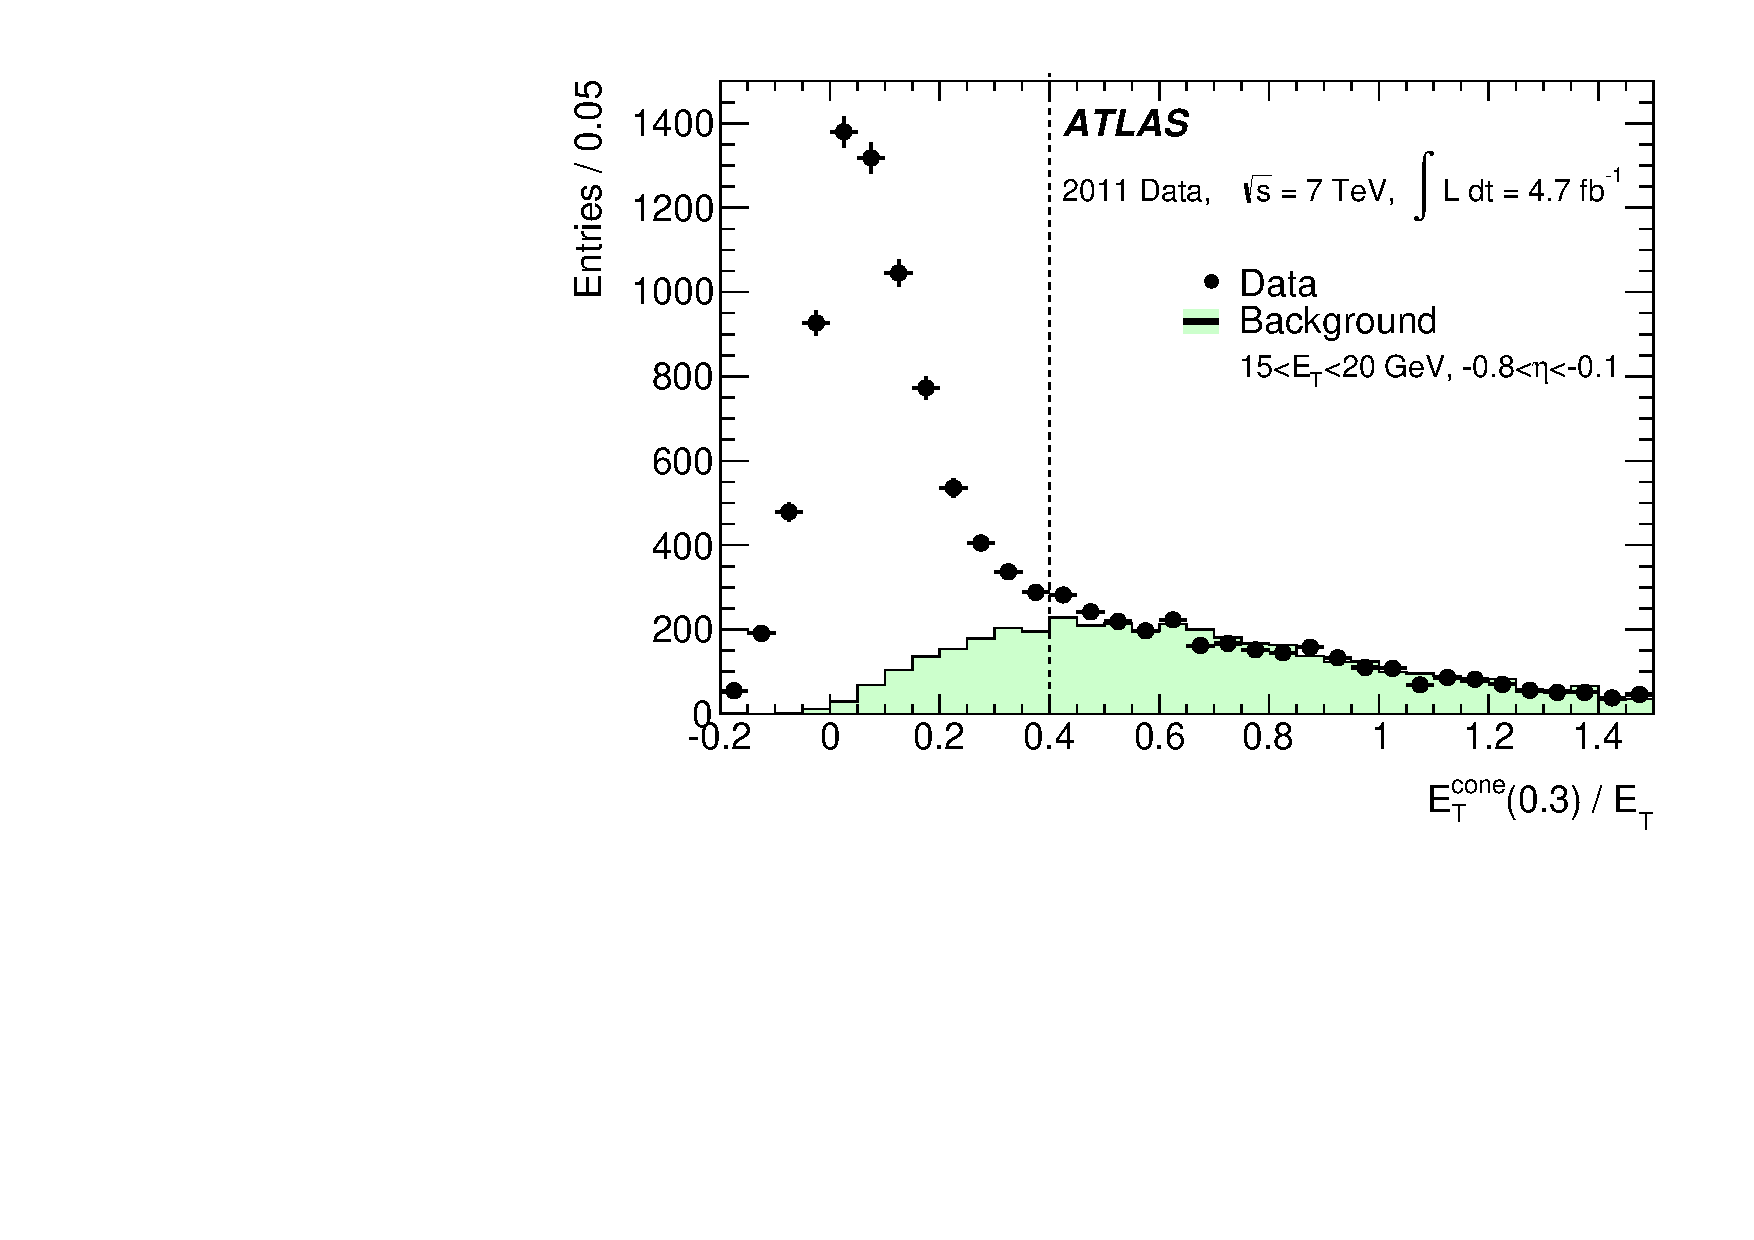
\includegraphics[width=0.45\textwidth]{figures/eff_rec_id_bg_a.pdf}}
\subfigure[\Zee]{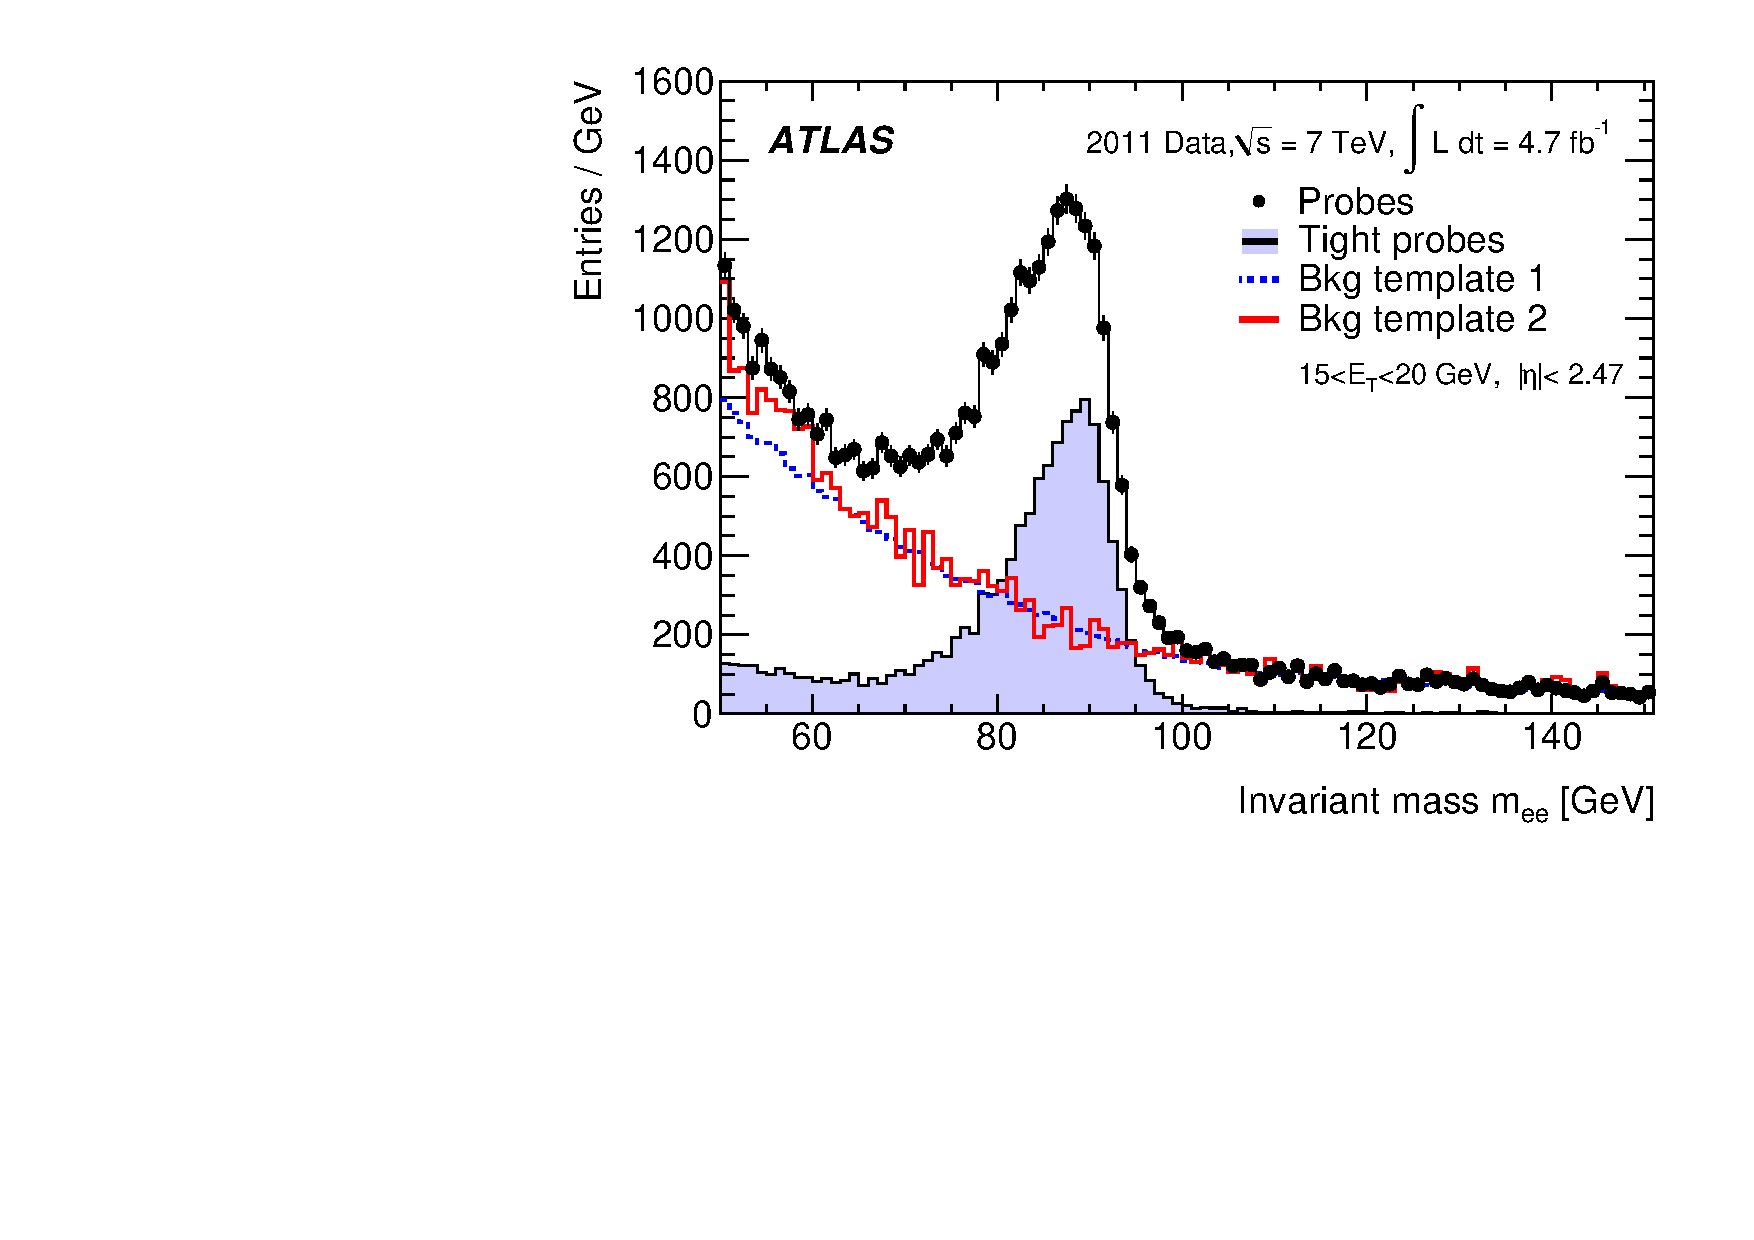
\includegraphics[width=0.45\textwidth]{figures/eff_rec_id_bg_b.pdf}}
\subfigure[$J/\psi \to ee$ prompt]{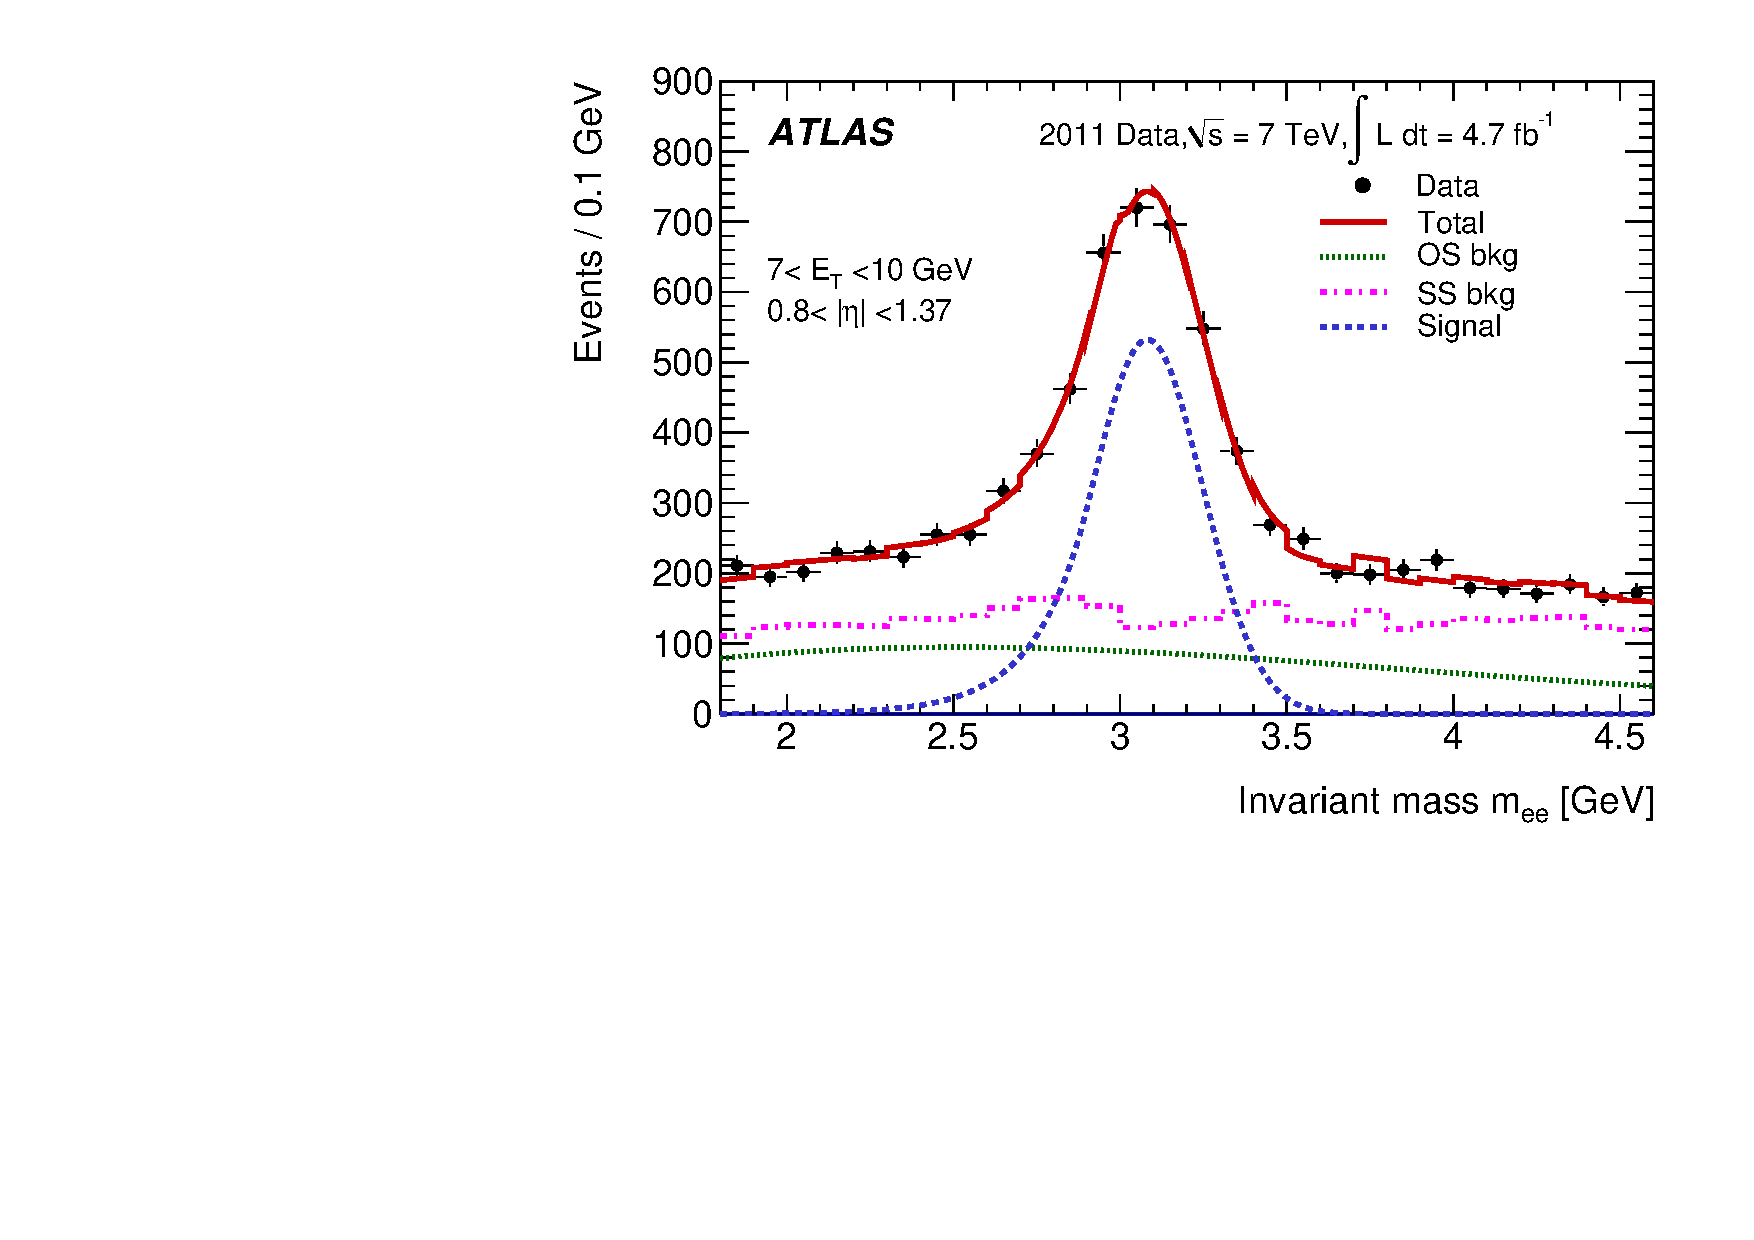
\includegraphics[width=0.45\textwidth]{figures/eff_rec_id_bg_c.pdf}}
\subfigure[$J/\psi \to ee$ non-prompt]{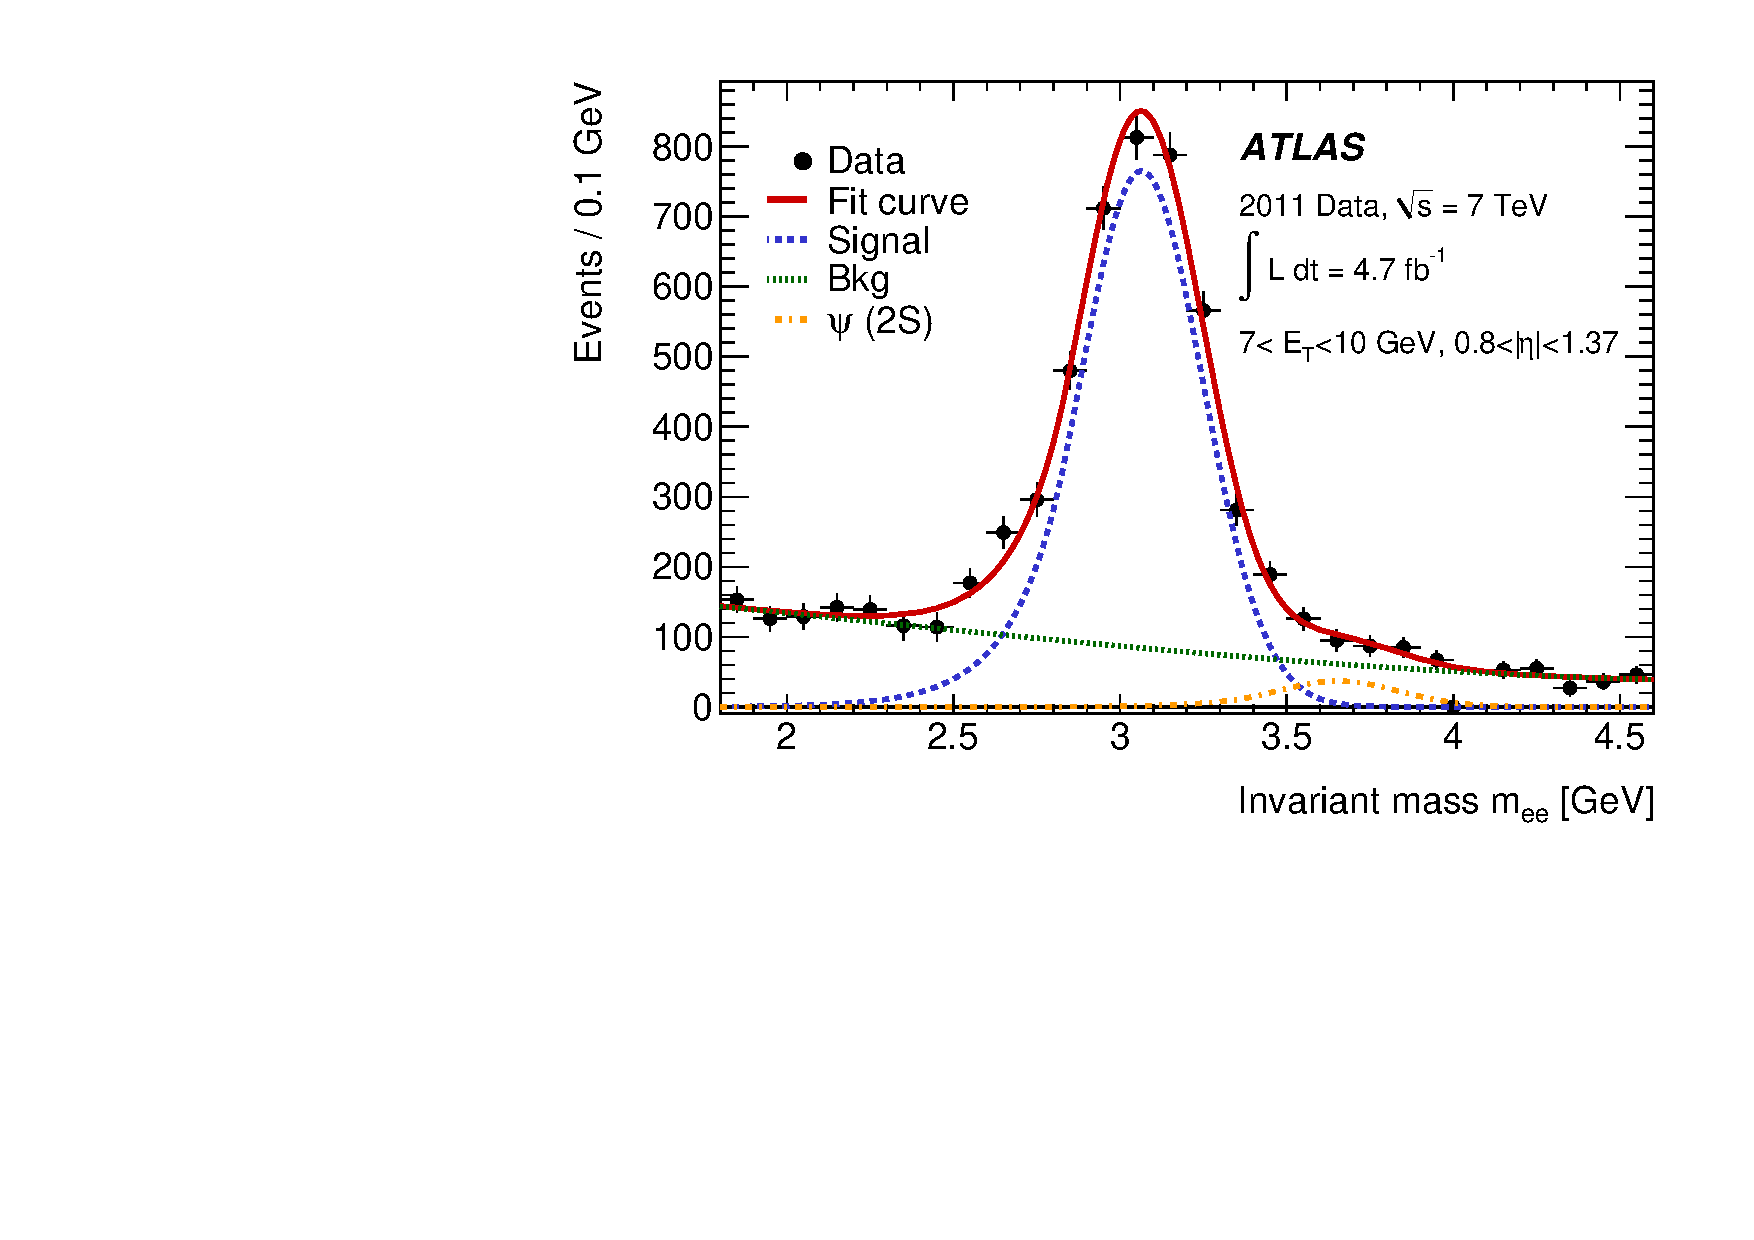
\includegraphics[width=0.45\textwidth]{figures/eff_rec_id_bg_d.pdf}}

\caption[Background estimation for different channels. (a) shows the $\et^{cone}(0.3)/\et$ variable of \Wenu\ events for probes (black dots) and normalized background template. The black dashed line shows the threshold. (b) shows two normalized background templates for \Zee, see text for details. (c) and (d) show backgrounds for short-lifetime (prompt) and long-lifetime (non-prompt) $J/\psi \to ee$ events respectively, being decomposed to various components.]{Background estimation for different channels. (a) shows the $\et^{cone}(0.3)/\et$ variable of \Wenu\ events for probes (black dots) and normalized background template. The black dashed line shows the threshold. (b) shows two normalized background templates for \Zee, see text for details. (c) and (d) show backgrounds for short-lifetime (prompt) and long-lifetime (non-prompt) $J/\psi \to ee$ events respectively, being decomposed to various components.~\cite{lib:elec_reco}}
\label{fig:eff_rec_id_bg}}
\end{figure}

For the uncertainties calculation, the shifting of various parameters is applied to all channels and the resulting shift in the efficiencies is observed. For the \Wenu\ events the thresholds for the $\et^{miss}$ and $m_{t}$ cuts are shifted, and the width of the cone for the discriminating variable is alternated to $0.4$. For the resulting $\sim$80 samples the backgrounds are then evaluated using the same method, and the resulting spread of the efficiencies is calculated. For the samples used the signal/background ratio distribution in the signal region exhibits an RMS (Root Mean Square) of 30\% at low \et\ (15-20~GeV) and 25\% at high \et\ (35-40~GeV). For the \Zee\ events the different mass-windows is used along with some alternative criteria for the tag electron. Both background templates are used, and in case of the isolation template the radius of the cone is also shifted, which gives in total about 120 samples. The S/B ratio distribution exhibits an RMS around 10\%. For the $J/\psi \to ee$ channel the isolation criteria was shifted for the tag electron as well as the high TRT requirement. The varying mass window and the same sign cut are also used to produce a total of 76 and 52 samples for prompt and non-prompt events respectively, with RMS around 30\%.

Since the events are statistically independent, their combination is used to produce the final results. Since it is data-to-MC ratio (which are scale factors, SFs) we are interested in, we can disregard the effects of the resolution or bin migration, since it will affect both data and MC similarly, and won't change the ratio. A global $\chi^{2}$ minimization was used to calculate the SF for every particular bin, in 2D \pt-$\eta$ binning. The formula for each bin is as follows:
\begin{equation}
\chi^{2} = \sum_{i,k} \frac{\left[ \mu^{i,k} - \mathrm{SF}^{i} - \sum_{j} \gamma_{j}^{i,k}\mathrm{SF}^{i}b_{j} \right]}
  {\left( \delta^{i,k}_{\mathrm{sta}} \right)^{2} \mu^{i,k}\mathrm{SF}^{i} \left( 1 - \sum_{j} \gamma_{j}^{i,k}b_{j} \right) + \left(\delta^{i,k}_{\mathrm{unc}} \mathrm{SF}^{i} \right)^{2}}
  + \sum_{j} b_{j}^{2} \,,
\end{equation}
where $i$, $k$, and $j$ run  over  the  $(\et, \eta)$ bins, the three channels, and the correlated systematics, respectively. The variables $\delta^{i,k}_{\mathrm{sta}}$, $delta^{i,k}_{\mathrm{unc}}$, and $\gamma_{j}^{i,k}$ represent the relative statistical, uncorrelated, and correlated systematic uncertainties respectively. The nuisance parameters $b_{j}$ are  related  to  correlated  uncertainties,  which are  dominated  by  the  background subtraction uncertainties. The combined scale factors are given by $\mathrm{SF}^{i}$. The resulting scale factors for some bins are shown in Figure~\ref{fig:eff_rec_id_SFs}.

\begin{figure}
\center{
\subfigure[$15 < \et < 20$]{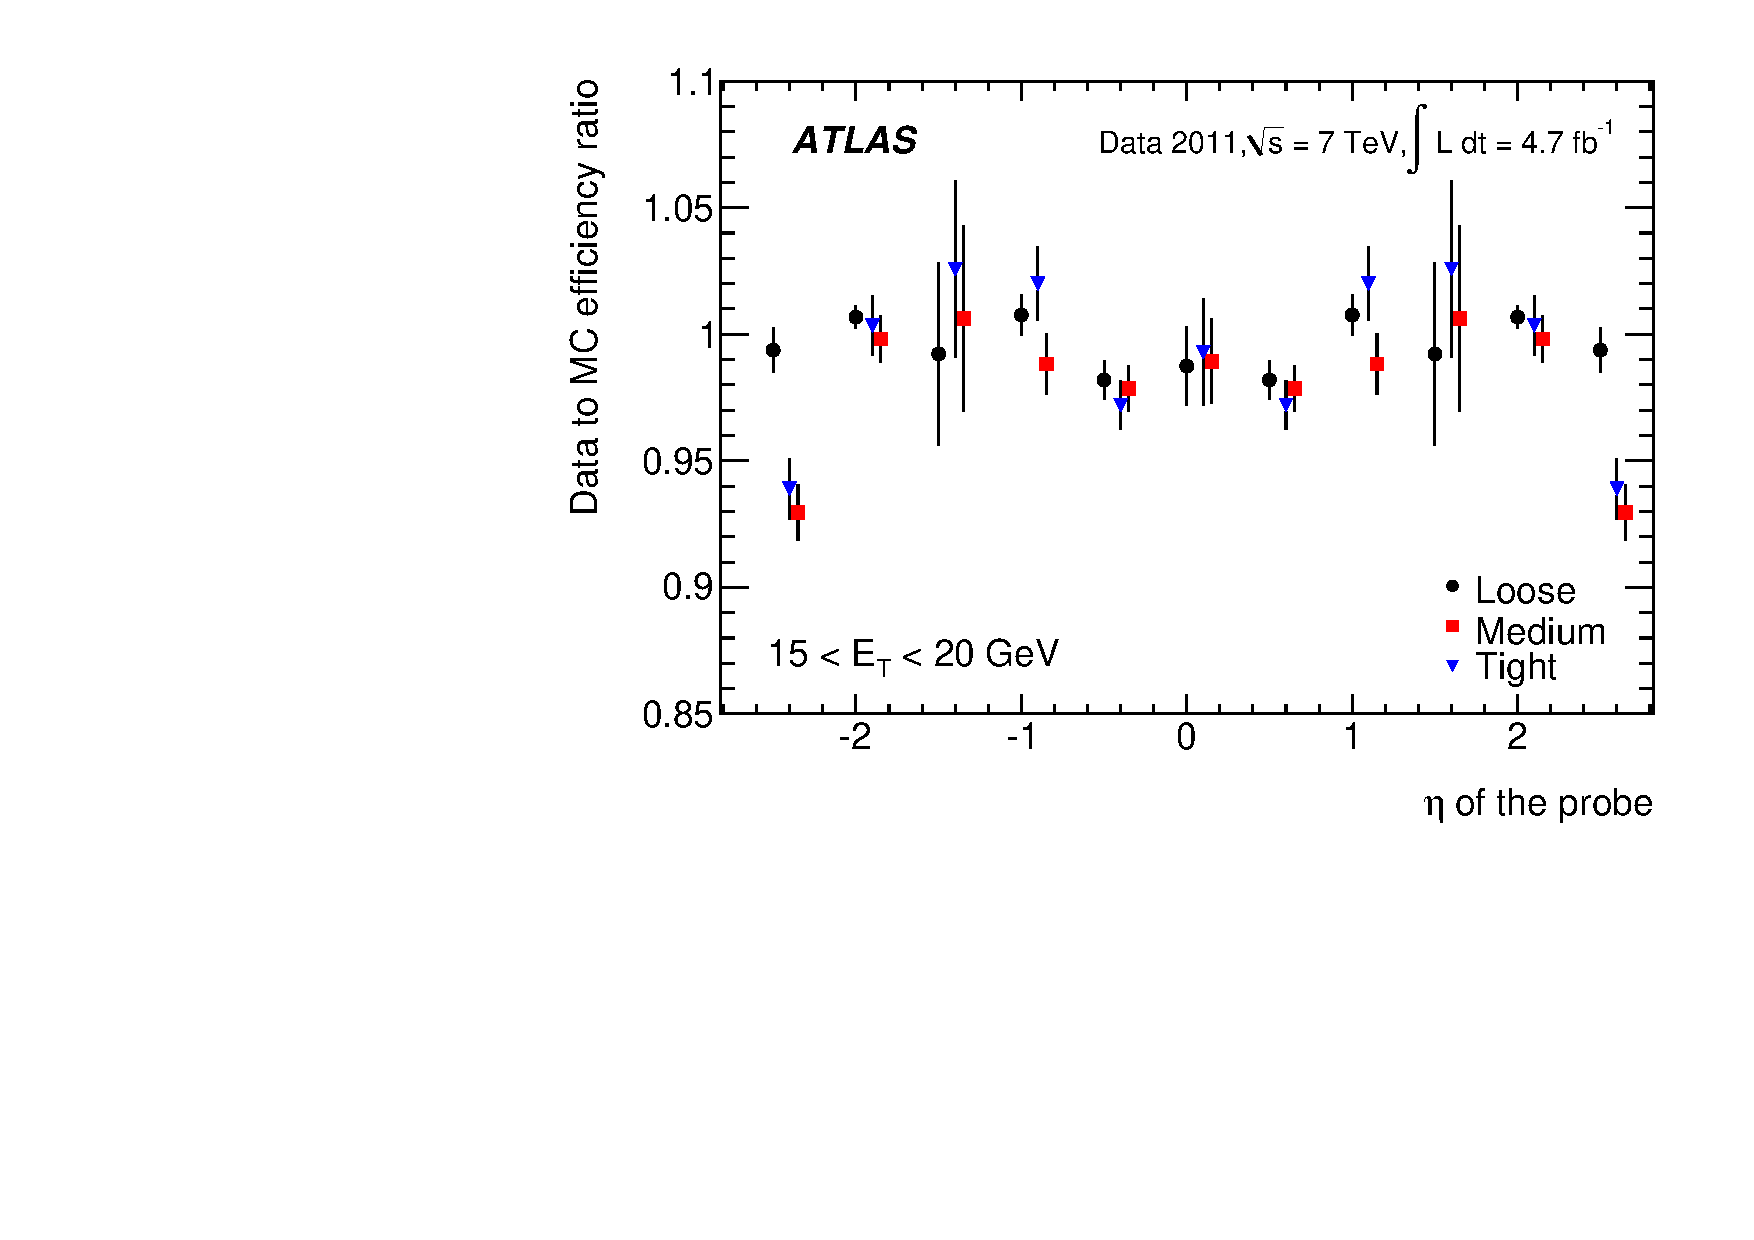
\includegraphics[width=0.45\textwidth]{figures/eff_rec_id_SFs_a.pdf}}
\subfigure[$35 < \et < 40$]{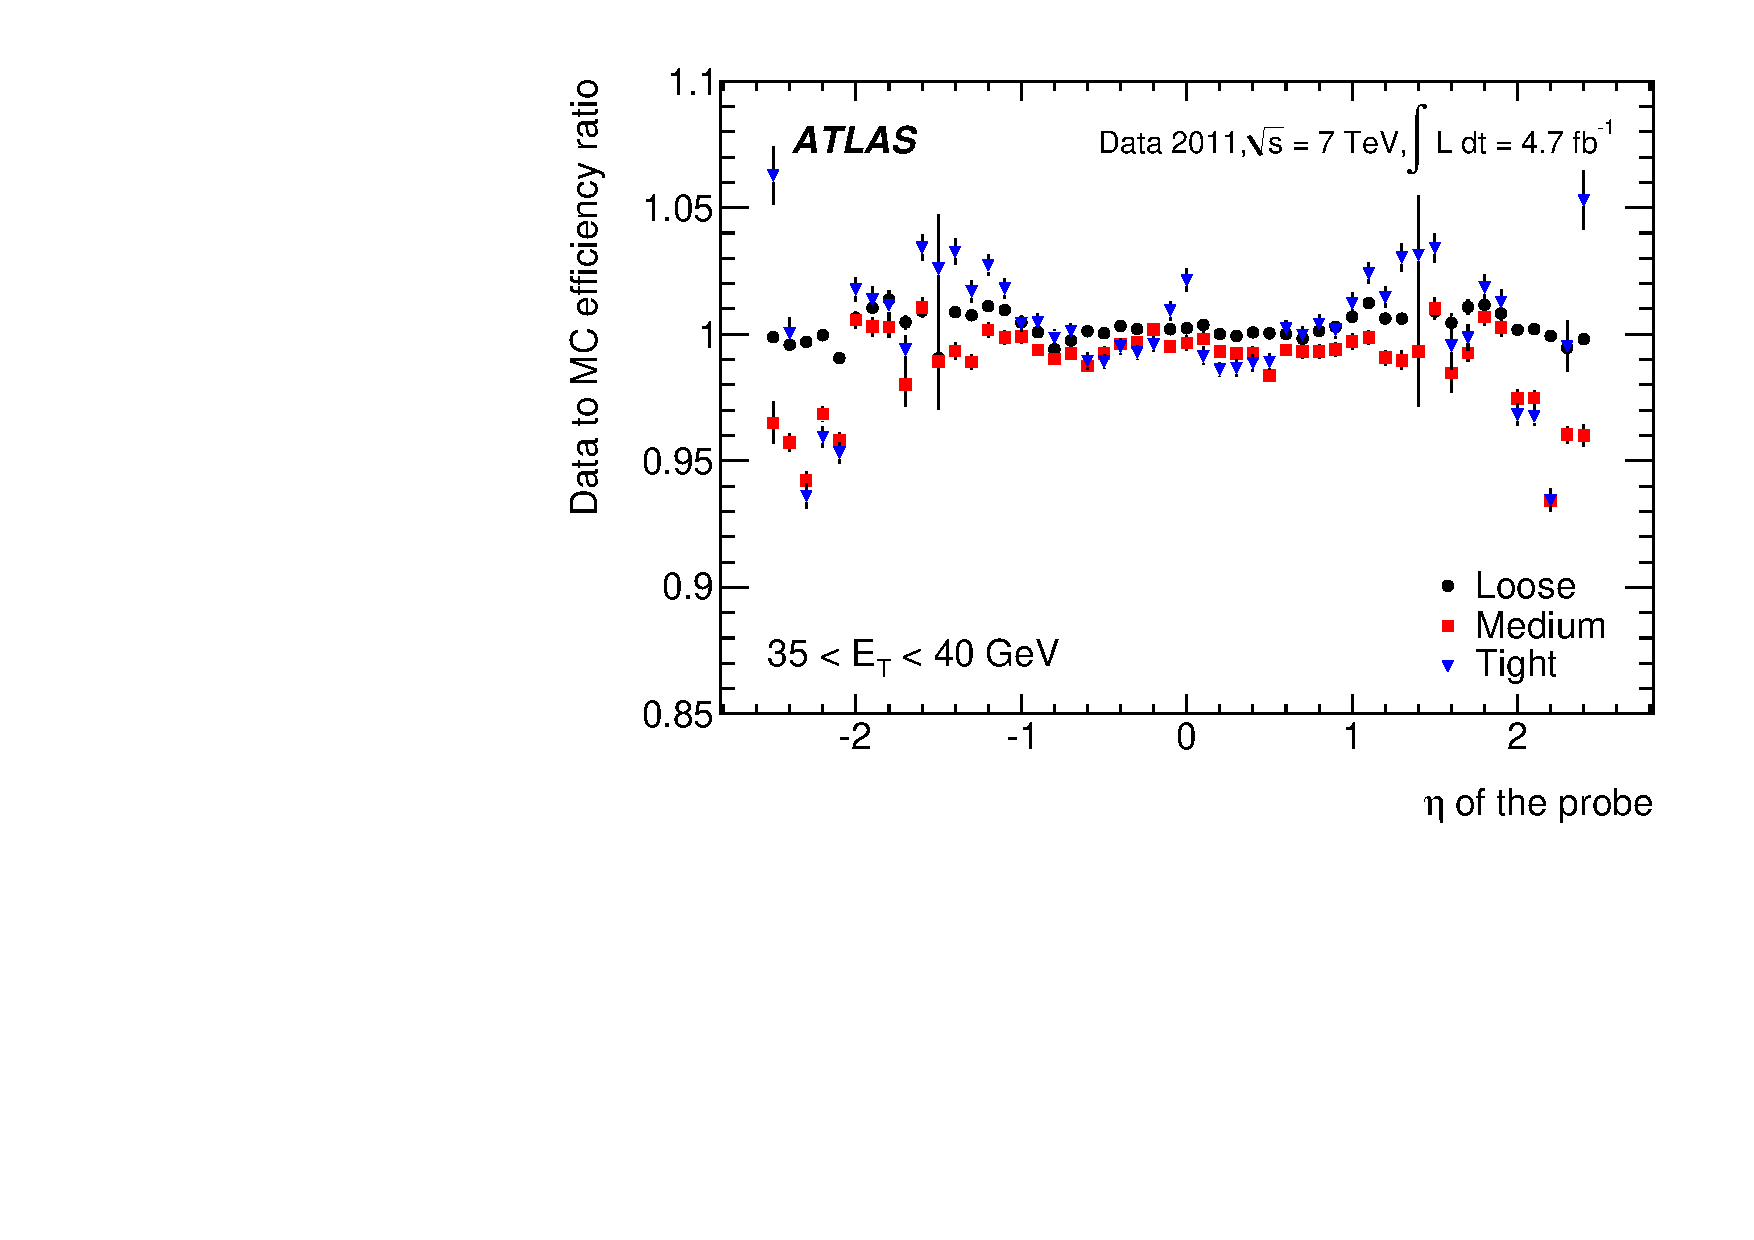
\includegraphics[width=0.45\textwidth]{figures/eff_rec_id_SFs_b.pdf}}

\caption[Examples of combined scale factors for the three identification criteria (loose, medium, tight) as a function of the pseudorapidity of the probe-electron $\eta$. Results are shown for different ranges of the probe electron energy. The error bars indicate the total uncertainties.]{Examples of combined scale factors for the three identification criteria (loose, medium, tight) as a function of the pseudorapidity of the probe-electron $\eta$. Results are shown for different ranges of the probe electron energy. The error bars indicate the total uncertainties.~\cite{lib:elec_reco}}
\label{fig:eff_rec_id_SFs}}
\end{figure}

\subsection{Forward electron identification efficiencies}

In the forward region of the calorimeters, the electron identification efficiency is measured with a \Zee\ central-forward sample  where  a  well-isolated $\et > 25$~GeV tag  electron satisfying the tight requirement is identified in the central region of the calorimeter and the probe cluster with $\et > 20$~GeV is found in the forward region. As an additional cut the low $\et^{miss}$ is required for the event candidates to suppress the contributions from \Wenu\ events.
The invariant mass $m_{ee}$ is fitted by the Crystal Ball function convoluted with a non-relativistic Breit-Wigner function with fixed $Z$ width to model the signal, and a Landau function to model the background in a mass window of $55 < m_{ee} < 130$~GeV. The S/B ratio is $\sim$7 for the outer EMEC and $\sim$5 for the FCAL. The various shifts to the tag requirements and to the fit parameters were performed to determine the amount of the systematical uncertainties, the resulting scale factors for selected bins can be seen in Figure~\ref{fig:eff_rec_id_forward_SFs}.

\begin{figure}
\center{
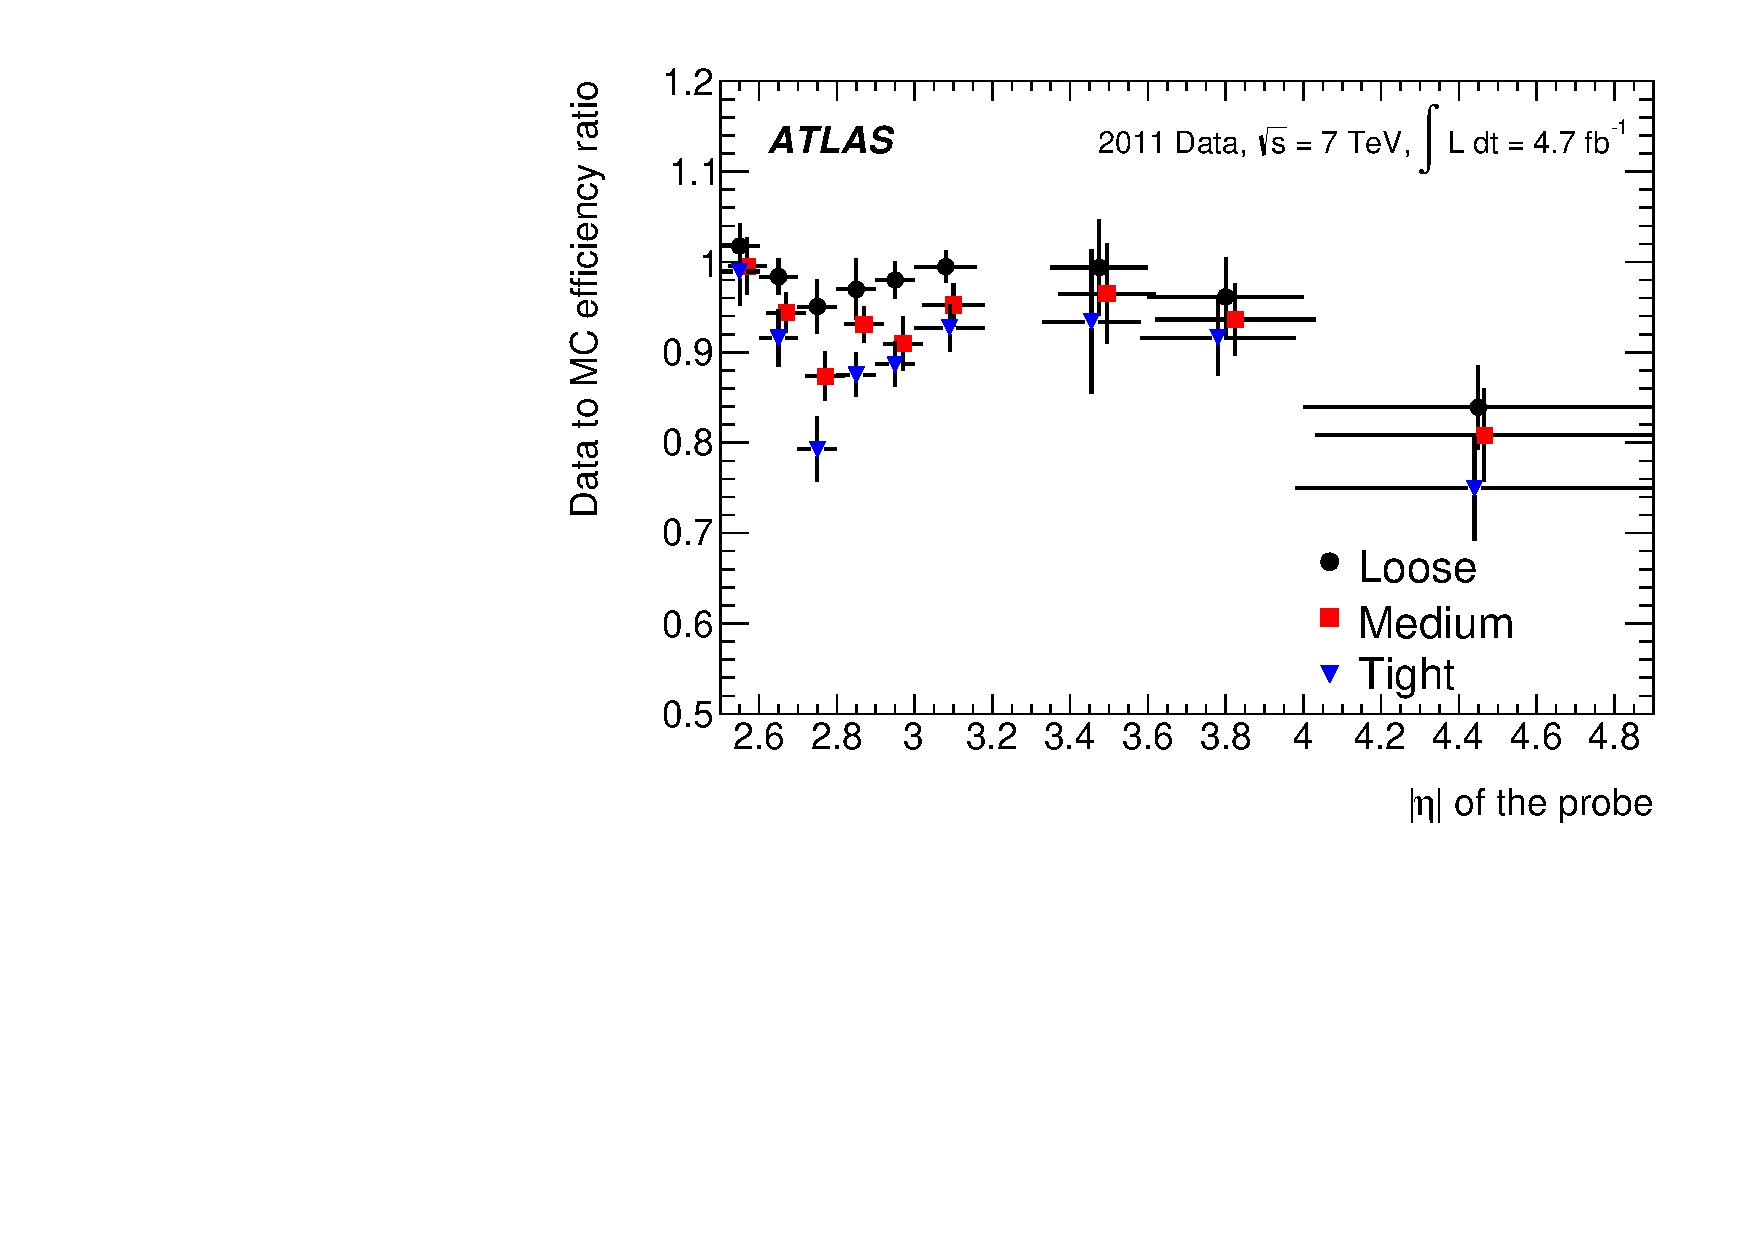
\includegraphics[width=0.5\textwidth]{figures/eff_rec_id_forward_SFs.pdf}
\caption[The scale factors for the forward electrons with $\et > 20$~GeV. The error bars correspond to the total uncertainties.]{The scale factors for the forward electrons with $\et > 20$~GeV. The error bars correspond to the total uncertainties.~\cite{lib:elec_reco}}
\label{fig:eff_rec_id_forward_SFs}}
\end{figure}


\subsection{Reconstruction efficiencies}

For reconstruction efficiency measurements the events from the \Zee\ channel are used for both central and forward electrons. As discussed in Section~\ref{sec:Rec_elec} the algorithm for the forward electrons is much more complex and gives an efficiency of about 97\% at 7~GeV and $\sim$99\% at 15~GeV. For the higher energies the efficiency of it is matched by that of the track reconstruction and cluster-track matching algorithms.

Efficiency values were measured for three samples:

\begin{itemize}
\item All reconstructed electron candidates in \Zee\ channel;
\item All the same electron candidates, but with additional requirement of the quality of the matching track, to match with the $J/\psi \to ee$ conditions described above;
\item All reconstructed electron candidates with additional requirements on hadronic leakage and the track quality to match with the \Wenu\ conditions described above.
\end{itemize}

The conditions for these measures follows that of the identification closely, except for the corrections for the photon conversions: the photons are included in the denominator when calculating the efficiency, provided they satisfy all the requirements. Naturally, that also means that the opposite sign requirement also doesn't apply.

For the background evaluation the same technique is applied: the background template is constructed using the inversion of several ID cuts (at least two from the loose ID not counting the ones dealing with the track) and failing the isolation requirement, and then normalized to the data in the high-mass region ($110 < m_{ee} < 250$~GeV).

The three samples together with the variations obtained from the variations of the background thresholds are used to find the systematic uncertainties with the same method as used in the identification efficiency calculation.

The resulting efficiencies can be seen in Figure~\ref{fig:eff_rec}. It can be seen that the systematical error increases greatly at $\et < 20$~GeV.

\begin{figure}
\center{
\subfigure[Reconstruction efficiencies]{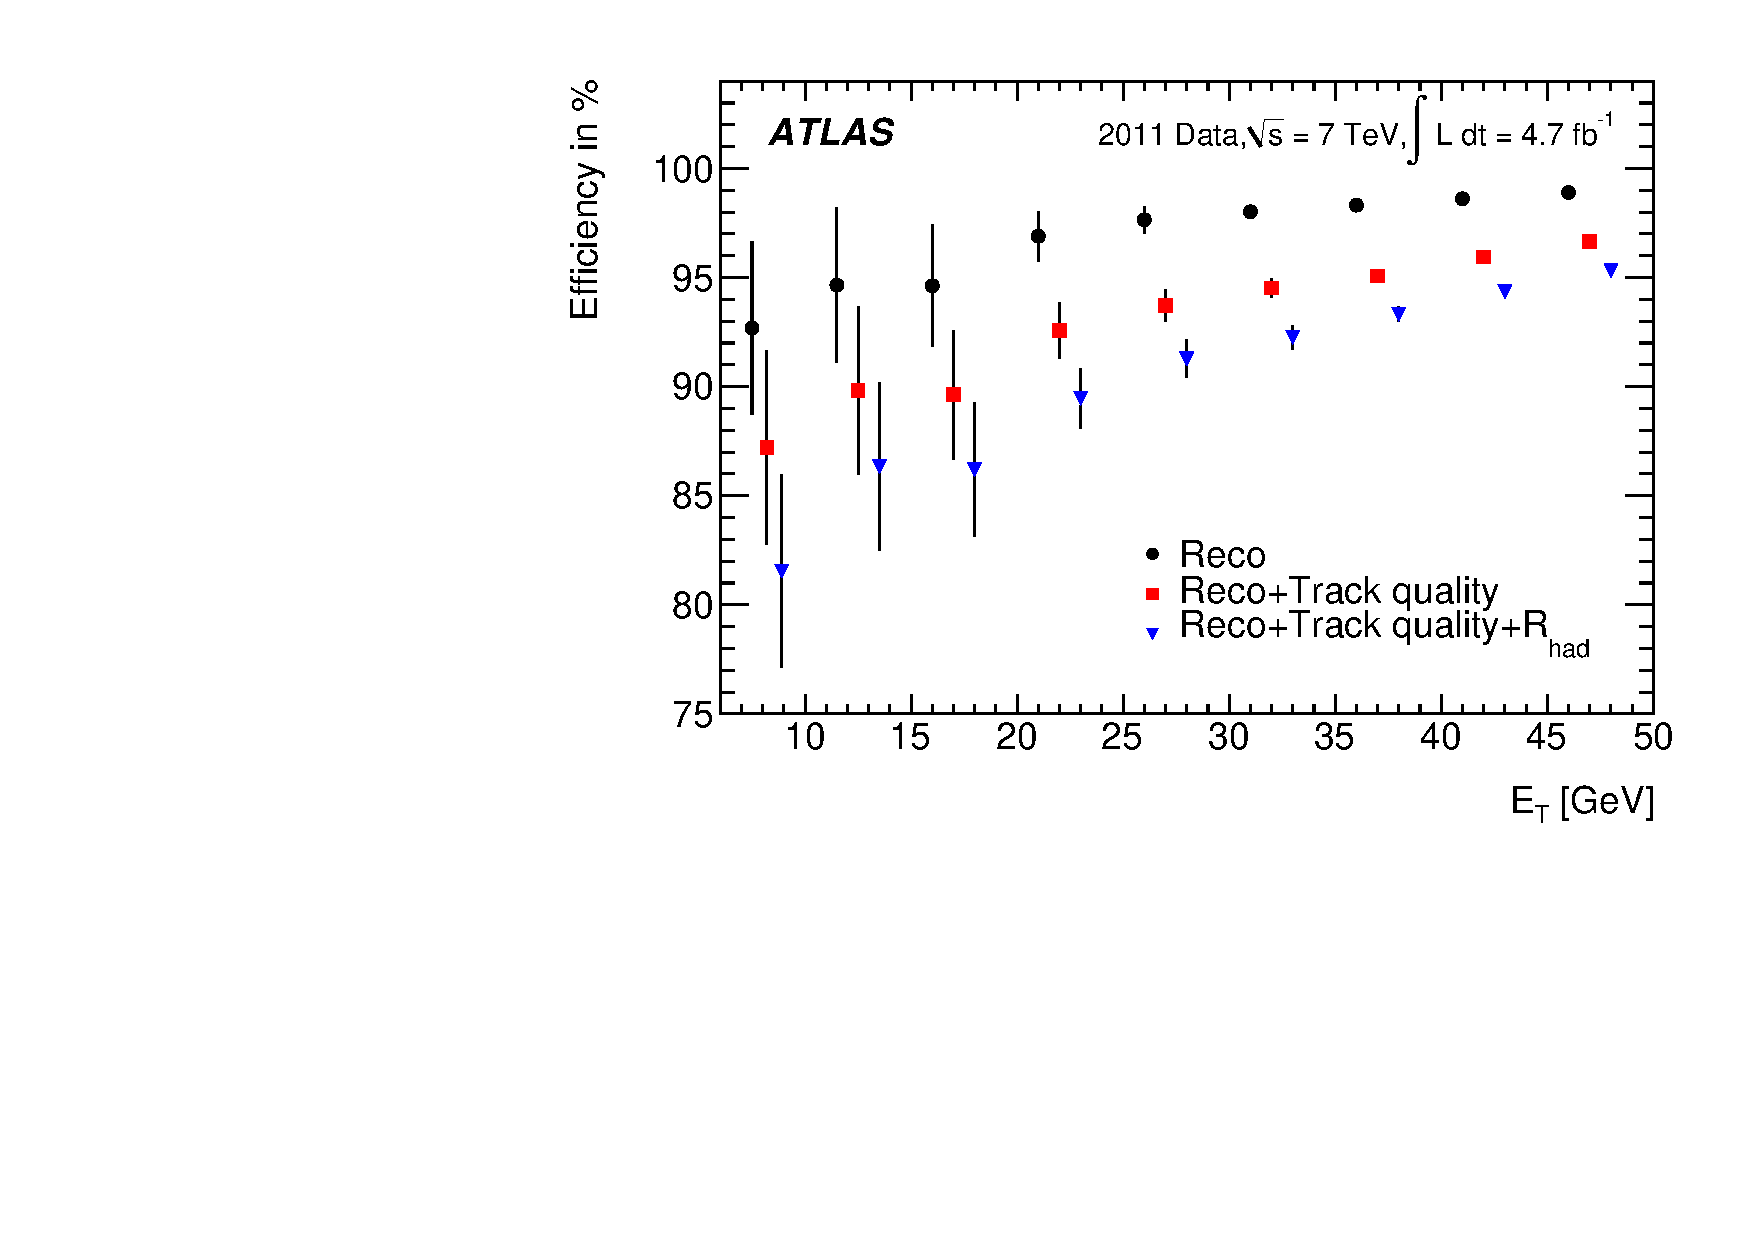
\includegraphics[width=0.45\textwidth]{figures/eff_rec_a.pdf}}
\subfigure[Systematical and statistical uncertainties]{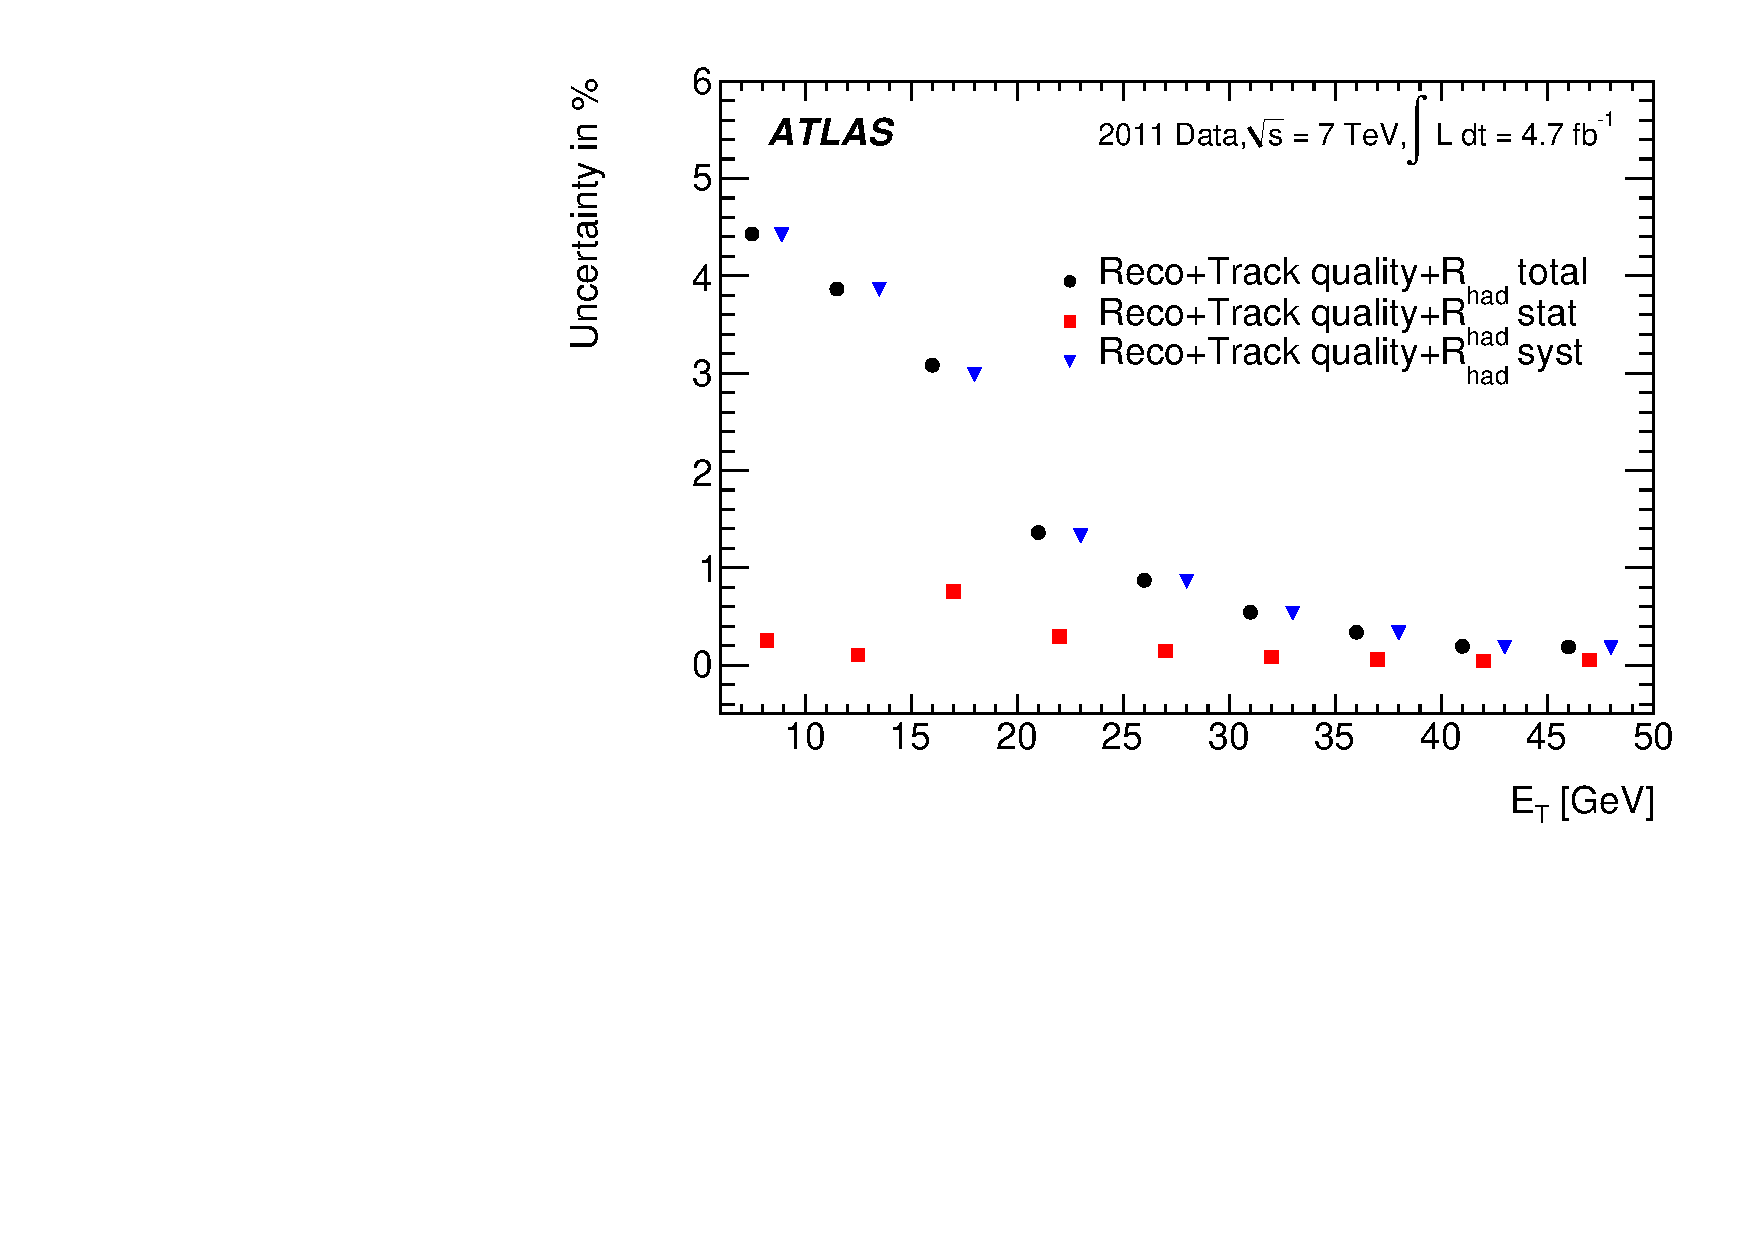
\includegraphics[width=0.45\textwidth]{figures/eff_rec_b.pdf}}

\caption[Reconstruction efficiencies for the central electrons, the error bars represent the total uncertainty, which can be seen fully in (b).]{Reconstruction efficiencies for the central electrons, the error bars represent the total uncertainty, which can be seen fully in (b).~\cite{lib:elec_reco}}
\label{fig:eff_rec}}
\end{figure}

\section{Isolation efficiency}

In the central-forward event selection of \Zee\ analysis the two additional isolation cuts are used in order to reduce the amount of the background: Iso98\et$^{\mathrm{cone20}}$ and Iso97\pt$^{\mathrm{cone40}}$ one being for the track and the other for the cluster. The efficiency of the isolation is thus the fraction of the electrons that pass this additional cut:
\begin{equation}
\varepsilon_\mathrm{Iso} = \frac{N_\text{probe with Iso} }{ N_\text{all probe} }, \;\;\;\;
\delta \varepsilon_\mathrm{Iso} = \frac{\sqrt{(1-2\varepsilon) \delta N_\text{probe with Iso}^2 + \varepsilon^2 \delta N_\text{all probe}^2}}
                                {N_\text{all probe}},
\end{equation}
where $\varepsilon_\mathrm{Iso}$ is the efficiency, and $\delta \varepsilon_\mathrm{Iso}$ is the corresponding statistical error.

The measurement was done with the \Zee\ sample with the same setup, with the \pt\ cut of the probe electron being lowered to 15~GeV and mass window reduced to $80 < m_{ee} < 100$~GeV to remedy the increased background. The remaining background is negligible (less than $0.1$\%).

The systematical error evaluation was done by shifting the mass window in the same way as the calculation of the trigger efficiencies, and by increasing the \pt\ cut for the tag electron to 24~GeV. The resulting efficiencies can be seen in Figure~\ref{fig:eff_iso_SFs}.

\begin{figure}
\center{
\subfigure[Isolation scale factors]{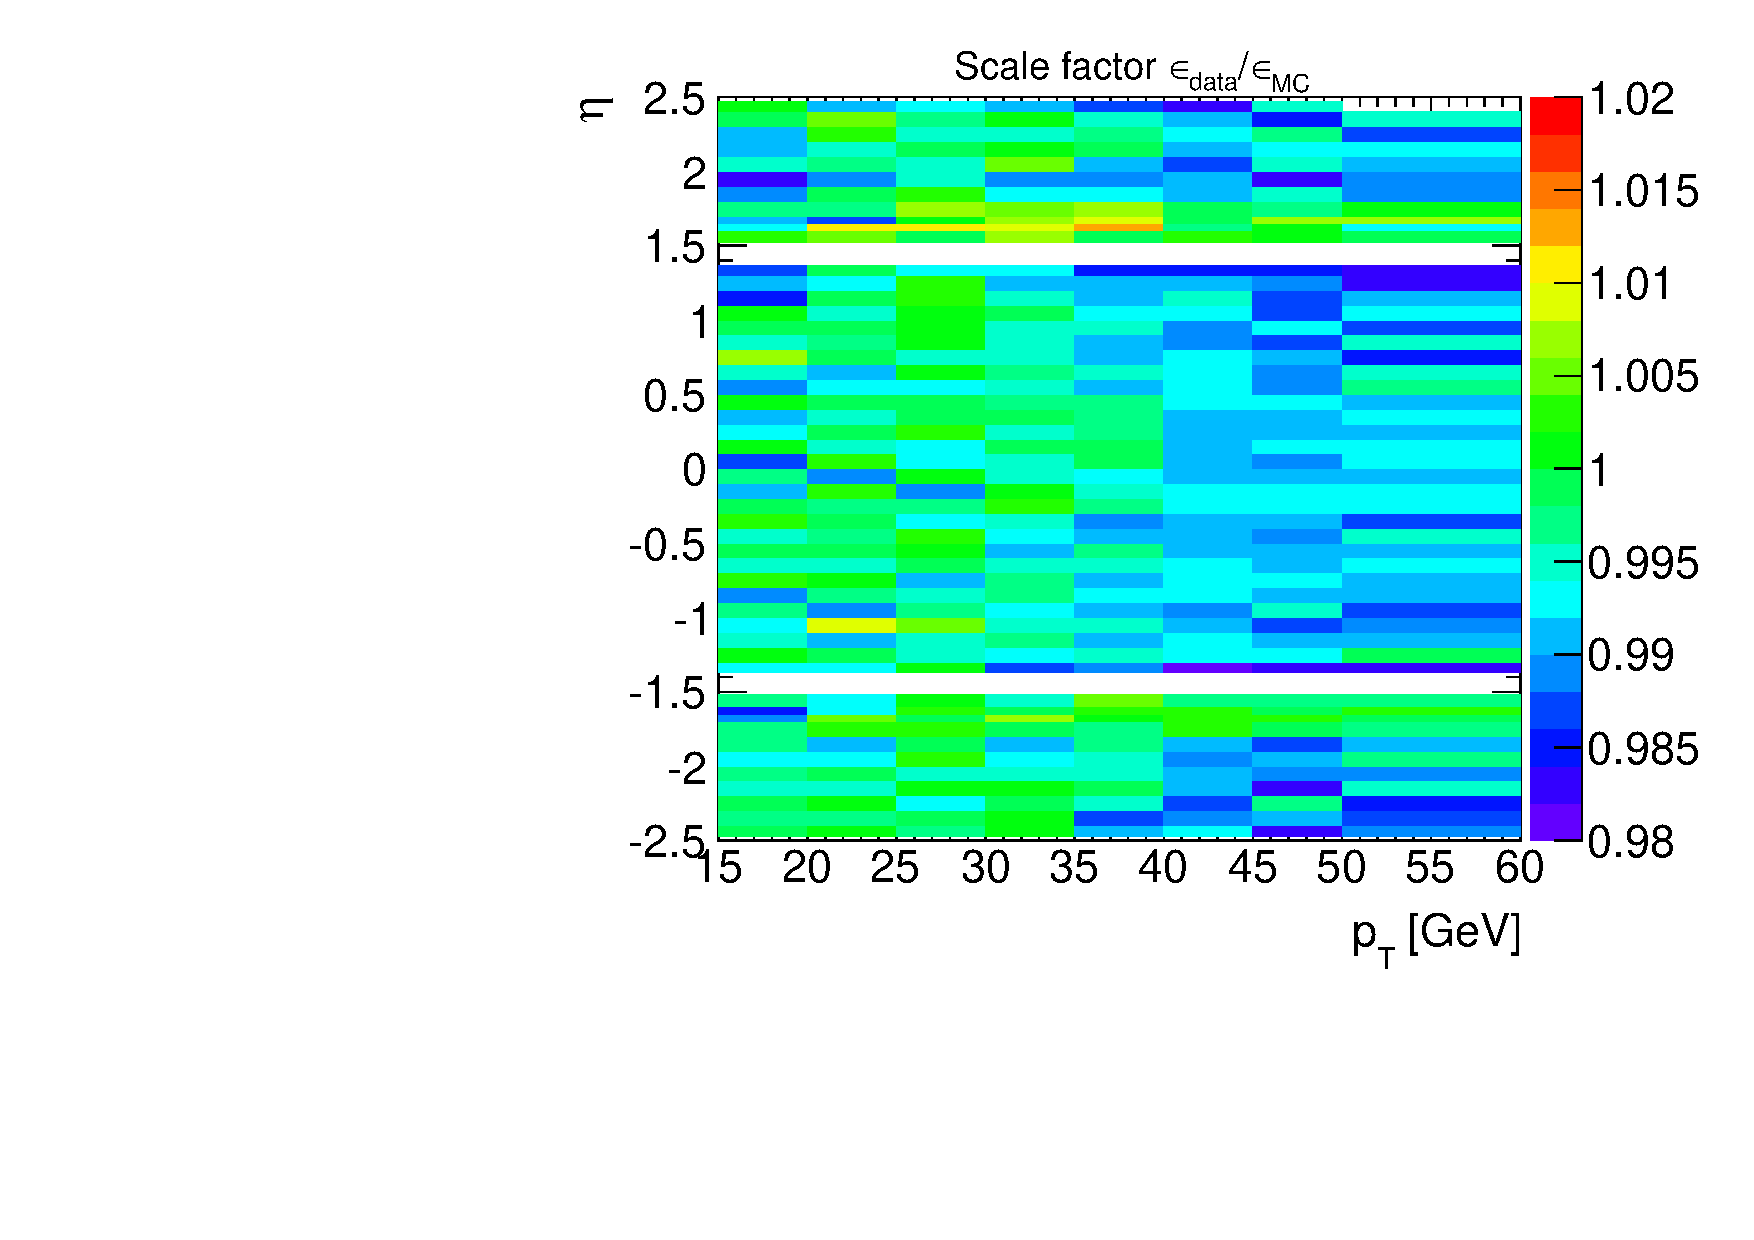
\includegraphics[width=0.45\textwidth]{figures/eff_iso_SFs.pdf}}
\subfigure[Statistical uncertainties]{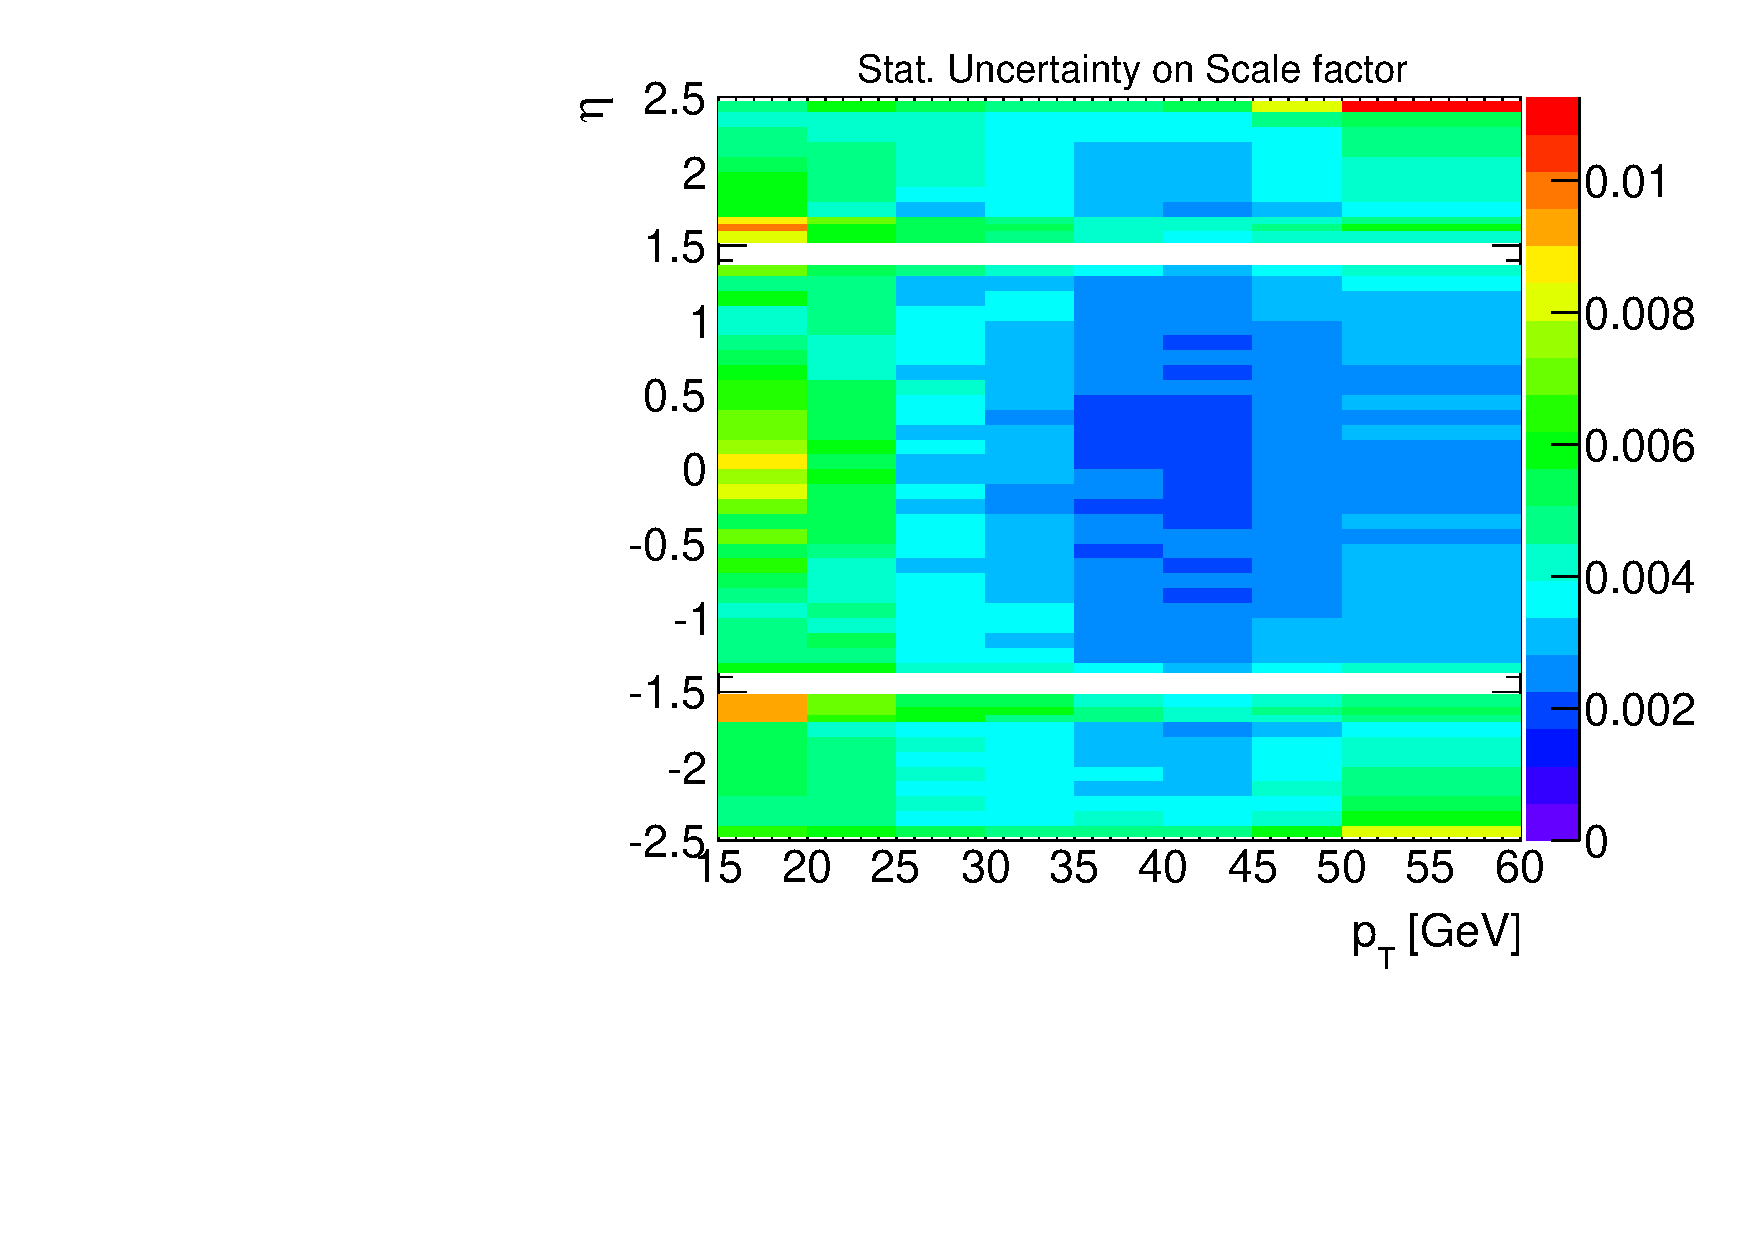
\includegraphics[width=0.45\textwidth]{figures/eff_iso_unc.pdf}}

\caption{Scale factors for the isolation efficiencies for the 2011 data together with statistical uncertainties in 2D binning by \pt\ and $\eta$. The plots were made using the \Zee\ MC samples with standard CC analysis cuts with the additional requirements on electron ID from the CF analysis.}
\label{fig:eff_iso_SFs}}
\end{figure}
